In the motion model, media components are parts of a larger media experience,
explicitly designed for external control. Component synchronization thus
involves a media component and an external motion object. The media component
synchronizes itself precisely relative to the motion. Relative synchronization
between media components connected to the same motion is achieved by
implication.

This section gives an introduction to component synchronization on the Web.
Synchronization of HTML5 media elements is covered. This serves as a case-
study for integrating established media frameworks into the motion model. In
addition, feasibility of the approach is demonstrated with respect to
synchronization quality. The section also covers development of custom media
components, focussing on synchronization (sequencing) of timed data (e.g.
subtitles, tracks, scripts, logs or time series). First though, component
synchronization is introduced by defining a basic pattern and some conventions.

\subsection{Basic Pattern}
\label{sec:pattern}

Consider a simple media component in a Web page. The media component has
access to two resources, media \textbf{data} and \textbf{motion}. Media data
is organized according to a timeline, and motion represents movement along
this timeline. Through its \textbf{UI} (user interface), the media component
may present \textbf{output} (e.g. pixels on screen, audio, vibration) and
receive \textbf{input} (e.g. key-presses, touch or mouse-events, camera, mic).

In these terms, the goal of component synchronization is simple: Given media
data and motion, generate the correct output at all times. To reach this goal,
implementations of component synchronization often follow a similar pattern.

\runinhead{Core processing loop:} 

Media components typically operate by repeating a core processing step:
\begin{enumerate}
\item{query the motion for current position (media offset)}
\item{identify the piece of media data that corresponds to current position}
\item{refresh the UI accordingly}
\end{enumerate}

For continuous media this core processing step is typically repeated at a
fixed frequency. For media components that visualize discrete media, the core
processing step is either run periodically (animation), or triggered by
timeout. In addition, three types of events interrupt the basic operation of
the media media component.

\runinhead{Motion change event:} 

Media components support media control by reacting to motion change events.
When position and/or velocity changes, internal state such as buffers and
schedules may have to be re-initialized, before the core processing step can
be run again. If paused (zero velocity), the media component runs its core
processing step once, and then terminate the core processing loop. If velocity
changes from zero to non-zero, the core processing loop must be started again.

\runinhead{Data change event:}

Some media components work with dynamic data sources, i.e. media data that may
change during presentation. This could be a live stream of timestamped
comments, or a time series from a live sensor. Media data may be added,
removed or modified. Modifications may imply re-positioning of data on the
timeline. In any case, media components must react by adjusting their internal
state accordingly, and run the core processing step.

\runinhead{Input (UI or API):} 

Interactive media components receive user input through UI events or API
methods. User input corresponding to media control requests must be forwarded
to the motion (causing motion change events by implication). This ensures that
control applies to all media components connected to the same motion. Other
types of user input trigger operations on the data model (causing data change
events by implication).

\subsection{Conventions}

In addition to the basic pattern, the motion model also defines a few
conventions for component synchronization.

\runinhead{Motion is the master:}

A distinctive feature of component synchronization is that the external motion
is not sensitive to the internal state of any media component. For instance,
motion might describe playback while a particular media component still lacks
data. If so, the media components should not halt the presentation until data
is ready. Instead, it must implement a reasonable behavior, given the
circumstances. For example, media components may adapt by buffering data
further ahead, changing to a different data source (e.g. lower bitrate) or
even changing to a different presentation mode (e.g audio only). This way,
playback may continue undisturbed and media components may join in as soon as
they are able to. This is particularly important in multi-device scenarios,
where a single device with limited bandwidth might otherwise hold back the
entire presentation. If the availability of a particular media component is
indeed essential to the media experience, this should instead be solved in
application-specific code, by pausing and resuming the external motion.

\runinhead{Reference point:}
\label{sec:referencepoint}
Media components synchronize their internal operations relative to an external
motion. However, if internal operations are subject to non-negligible delays
before they take effect, the resulting experience may still be incorrectly
synchronized. Though this problem is not specific to the motion model, it
still threatens the main ambition; that synchronization is simply a
consequence of connecting multiple media components to the same motion. To
avoid this, media components must compensate for delays internally by
scheduling actions earlier. This assumes that media components know or are
able to estimate such delays.

More formally, the concept of reference point in media playback refers to the
point in time when timed media data take physical effect. In the motion model,
the external motion defines the reference point.


\subsection {Integrating media frameworks}
\label{sec:html5sync}

Integration of existing media frameworks in the Web platform (e.g. HTML5 media
elements~\cite{html5media}, WebAudio~\cite{webaudio},
WebAnimation~\cite{webanimation}) into the motion model would be very
attractive. Currently though, they do not support internal synchronization, so
external synchronization is the only option. This means that synchronization
must be implemented in JavaScript, using the relevant control primitives that
each framework defines.

As a case-study in integration, this section discusses synchronization of
HTML5 media elements (i.e. audio and video). Media elements have not been
designed for synchronization, so this is not an optimal basis for evaluating
motion-based synchronization. Still, by identifying the capabilities and
limitations of current media elements, at least a baseline indication may be
provided. Likely, native support for synchronization will yield a significant
improvement.

The goal of motion-based synchronization of media elements is to keep the
\emph{currentTime} property (i.e. media offset) equal to the position of the
motion at all times, at least to a good approximation\footnote{This definition
assumes that the currentTime property matches the reference point for AV
playback. In our experience, this assumptions turns out to be reasonably
sound, though this is not mentioned as part of the specification for HTML5
media elements. }. The available control primitives include \emph{play},
\emph{pause}, \emph{seekTo} and \emph{variablePlaybackrate}. SeekTo specifies
a new media offset, and variablePlaybackrate allows media playback to speed up
or slow down.

The main challenge for precise synchronization is that HTML5 media elements
operate in their own time frame. They may be requested to play at a specific
time, yet the precise scheduling of media playback is subject to various
internal delays, such as time consumption in initialisation procedures,
buffering, decoding and AV-subsystems. There is also player drift, meaning
that the effective playback rate is not exactly equal to the rate of the
system clock. Finally, all these details vary across different architectures,
browsers and media formats.

So, the general approach is simply to evaluate currentTime property
continuously, and try to rectify whenever the synchronization error grows
beyond a certain threshold. For larger errors seekTo is used. This is
typically the case on load, or after motion change events. Smaller errors are
rectified gradually by manipulating variablePlaybackrate. SeekTo is quite
disruptive to the user experience, so support for variablePlaybackrate is
currently required for high quality synchronization.

\runinhead{Implementation:}

MediaSync is a JavaScript library (part of Timingsr~\cite{timingsrc}) allowing
HTML5 media elements to be synchronized by motion. The library works by
monitoring the motion, and adjusting the media element when needed. The
MediaSync library targets usage across the most common Web browsers, so it is
not optimized for any particular scenario.

The first practical challenge involves the resolution and precision of the
media offset. The currentTime property is updated at a fixed frequency,
typically about 4Hz, which is the recommended frequency for the timeupdate
event. The MediaSync library only samples the currentTime property immediately
after this event. More importantly, when compared to the system clock, the
currentTime property typically fluctuates considerably between samples. As a
consequence, the MediaSync library collects a backlog of samples, from which
the true value of the currentTime value can be estimated, with improved
resolution. Building up this backlog requires some samples, so it may take
more than a second for estimates to stabilize.

Another issue relates to unpredictable time-consumption in media control
operations. For instance, seekTo(X) will change currentTime to X, but it will
require a non-negligible amount of time to do this, as both buffering and
internal processing may be required. The problem is that seekTo does not
compensate for playback during its execution, so it is always wrong, at least
in the context of synchronization. In other words, it aims for a fixed target,
when it should aim for a moving target. The MediaSync library compensates for
this by overshooting the target. Furthermore, in order to overshoot by the
correct amount, the algorithm collects statistics from every seekTo operation.
Surprisingly perhaps, this strategy works.

Finally, there are some issues that cannot be compensated in JavaScript. Not
every browser supports variablePlaybackrate, and some claim they do even if it
is broken. Furthermore, sometimes playback is required to start at a media
offset other that 0. If so, synchronization starts with seekTo, followed by
play. In this case, the issue with time-consumption in seekTo implies that
buffering starts with data that will not be needed. This works against the
important goal of quickly being able to join a synchronized media
presentation.


\runinhead{Evaluation:}

Two technical reports~\cite{syncreport1,syncreport2} document the abilities and
limitations of HTML5 media elements with respect to media synchronization, as
well the quality of synchronization achieved by the MediaSync library. In
short, for desktops, laptops and high-end smartphones, echoless audio playback
is expected both for video+audio and audio only. Smartphones, and embedded
devices such a ChromeCast, can be expected to provide frame accurate
synchronization. Target precision is generally achieved within 3 seconds. It
is also worth noting that measured results are consistent with human
observation. Echoless synchronization with the MediaSync library produces
various audio effects, like failing to hear one audio source, until volume
levels are changed and only the other audio source can be heard. Since these
effects are also achieved across browser types and architectures, this is a
strong indication that currentTime approximates the reference point
quite well (see Sect.~\ref{sec:referencepoint}).

\begin{figure}[h]
%\sidecaption
\centering
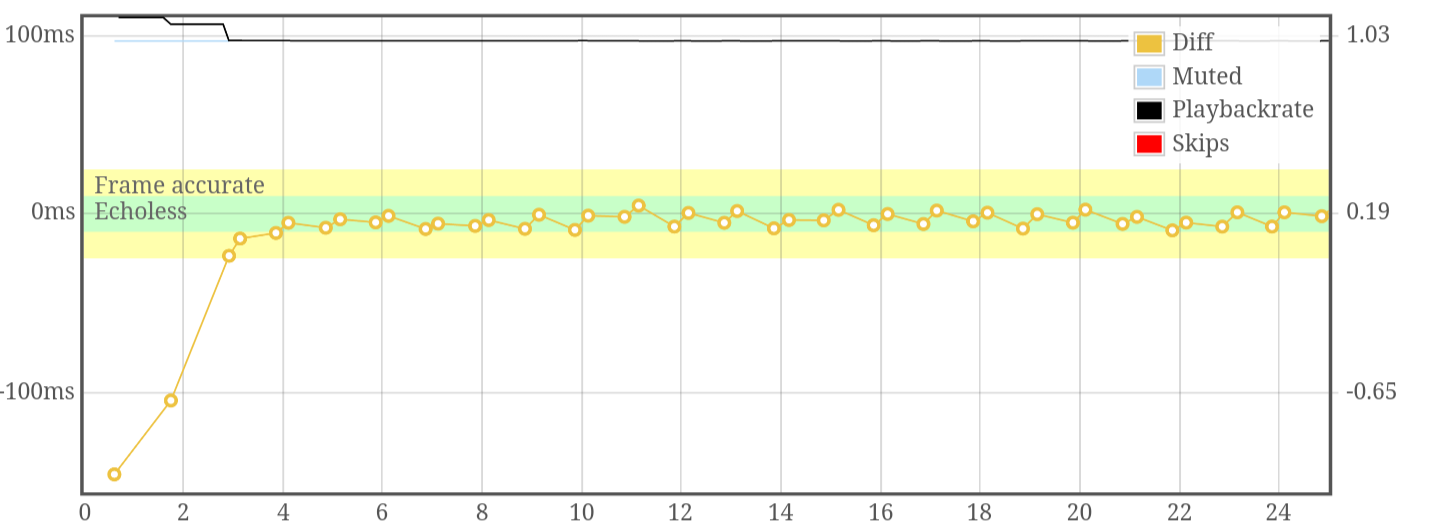
\includegraphics[scale=.23]{fig/android-video.png}
\caption{The figure illustrates an experiment with video (mp4) synchronization on
Android using Chrome browser. The plot shows currentTime compared to the ideal
playback position defined by motion. The green band (echoless) is +-10 millisecond and
the yellow (frame accurate is) +-25 millisecond. The media element enters frame accurate
playback after two seekTo operations, and converges on echoless using
variablePlaybackrate.}
\label{fig:videosync}
\end{figure}

Though echoless synchronization is generally achievable, there are always a
few combinations of architecture, browser and media format that pose problems.
Errors may also occur and vanish across software updates. To be able to
support echoless synchronization reliably across the board, standards must
include requirements for synchronization, and testing-suites must be developed
to ensure that those requirements are met. Ideally though, media
synchronization should be implemented natively in media elements. Given the
challenges faced by the MediaSync library, it is not unlikely that native
implementations would provide a significant improvement.

\subsection{Custom media components}

Custom media components are developed for applications specific media sources
and/or applications specific visualizations. Building a custom media component
is basically a standard exercise in Web development. For instance, development
may involve a data source (e.g. JSON data), UI ($<div>$ element in the DOM),
and some code (JavaScript) implementing the functions of the basic  pattern
(see Sect.~\ref{sec:pattern}). Still, the basic pattern includes challenges
regarding timing and synchronization that may be challenging, especially for
developers with limited time on their hands. Fortunately, much of this
complexity may be encapsulated and solved by generic programming tools. In
this section we focus on custom media components working with timed data (e.g.
subtitles, tracks, scripts, logs, time series), and demonstrate  how a
sequencer turns this into a trivial programing challenge.

\runinhead{Sequencer:}

Timed data typically involves items tied to points or intervals on a timeline.
Synchronized presentation (or visualization) of timed data then requires items
to be activated and deactivated at the correct time, in reference to the
motion.

\begin{figure}[h]
%\sidecaption
\centering
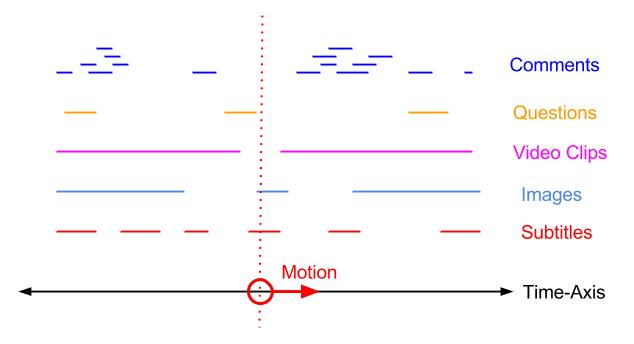
\includegraphics[scale=.4]{fig/sequencer.jpg}
\caption{Five data sources of timed data, with items tied to intervals on the timeline. Motion along the same timeline defines which items are active (vertical dotted line), and precisely when items will be activated or deactivated.}
\label{fig:sequencer}
\end{figure}


The Sequencer~\cite{sequencer} is a generic tool for precise activation and
deactivation of timed data, in reference to a motion. Web developers parse
media data and registers cues tied to points or intervals on the timeline. The
Sequencer is then responsible for emitting enter and exit events for those
cues, at the correct points in time. By associating callback function to those
events, Web developers may update visualizations at the correct time.

The sequencer fully supports the basic pattern of component synchronization.
It is directed by motion and supports all the flexibility of motion-based
media control, including skipping, reverse playback and acceleration. It also
supports dynamic changes to data. Cues may safely be added, removed or changed
at any time during media presentation. The Sequencer guarantees that emitted
enter and exit events are always consistent with the current state of the
motion, and the current state of media data (i.e. cues.). By operating on cues
instead of data, the Sequencer does not require a specific data format. Also,
the Sequencer is not tied to any predefined visuals, leaving Web programmers
to implement synchronized UI’s with the full power of the Web platform at
hand.

In short, the Sequencer constitutes an important building block for
development of custom media components. It encapsulates complexity related to
motion-based synchronization and dynamic data, and leaves Web developers with
two simple task; registering cues and implementing event listeners. By using
generic programming tools such as the Sequencer,  Web developers with little
expertise in media synchronization may develop precisely synchronized
visualization based on application specific data sources.

\runinhead{Sequencer API:}
The following code snippet outlines the Sequencer API. The
complete API documentation, example code and demos are available at the
Timingsrc~\cite{timingsrc} Website.

\begin{lstlisting}[caption=Sequencer usage example]
// sequencer constructor
var seq = new Sequencer(motion);
// add or modify cue
seq.addCue("key", new Interval(12.2, 14.4), "data");
// remove cue
seq.removeCue("key");
// register event handler
var enter = function(e){console.log("enter", e.key, e.data)};
var exit = function(e){console.log("exit", e.key, e.data)};
seq.on('enter', enter);
seq.off('exit', exit)
\end{lstlisting}

\runinhead{Implementation:}

The Sequencer is implemented as a JavaScript library, and open-sourced as part
of the Timingsrc programming model~\cite{timingsrc}. In the interest of
precisely synchronized activation and deactivation and low cpu consumption,
the Sequencer implementation is not based on frequent polling. Instead, the
deterministic nature of motion allow events to be calculated and scheduled
using setTimeout, the timeout mechanism available in Web browsers. Though this
mechanism is not optimized for precision, Web browsers may be precise down to
a single millisecond. Over the last years, the Sequencer has been used
extensively by our research group. Further details are presented in this
paper~\cite{sequencer}.


%\subsection{Summary}
%The motion model makes media synchronization very easy for Web developers,
%especially if popular media frameworks have already been integrated and
%made available as reusable, common-purpose media components. If not,
%developers may have to implement wrapper code for media frameworks
%themselves, or implement custom media components. Sequencing
%tools makes development of custom media components much easier.

